\chapter{DC Circuits}
\begin{comment}
\section{Introduction}

In this experiment you are going to construct a slide-wire potentiometer and use it to measure the electromotive force (emf) of a battery. The emf is a somewhat misleading term, since it does not refer to a force at all, but to the voltage (or energy per unit charge) made available by the battery. \myskip

You may be wondering why we cannot simply attach a voltmeter (device that measures voltage) to the battery and say that the voltage we read is the emf of the battery. The reason for this is because the battery has its own internal resistance, and when the voltmeter sends current through the battery to measure the voltage, the internal resistance of the battery affects the voltage measured. Therefore, in order to accurately measure the emf of a battery, we have to use a device that does not draw any current through the battery. The potentiometer is one such device that will accomplish this goal. \myskip

The potentiometer is also used to measure the small voltage across a thermocouple, which is a device used to determine temperature differences by measuring the thermal emf produced at the junctions of dissimilar metals. In this case, the thermal emfs cannot supply sufficient current to be measurable on an ordinary meter, so a potentiometer is used.

\section{Theory}

\subsection{Resistance of a uniform wire}

Consider a uniform wire of length $l$ and cross-sectional area $A$ with a potential difference $\Delta V = V_b - V_a$ maintained across it, as shown in figure \ref{fig:reswire}

\begin{figure}[h]
    \begin{center}
        %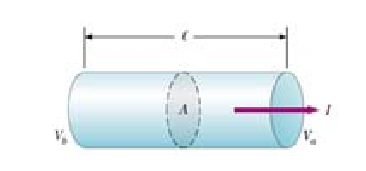
\includegraphics[width=0.25\textwidth]{./Exp2/pic/image1.png}
        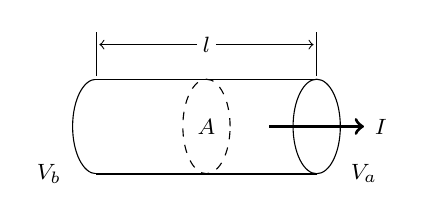
\begin{tikzpicture}[scale=0.4,font=\footnotesize]
            \draw (-3.5,1.5) -- (3.5,1.5);
            \draw (-3.5,-1.51) -- (3.5,-1.51);
            \draw (3.5,0) ellipse (0.75 and 1.5);
            \begin{scope}
                \clip (-4.5,1.5) rectangle (-3.5,-1.5);
                \draw (-3.5,0) ellipse (0.75 and 1.5);
            \end{scope}
            \node at (0,0) {$A$};
            \draw[dashed] (0,0) ellipse (0.75 and 1.5);
            \draw[very thick,->] (2,0) -- (5,0) node[right] {$I$};
            \draw (-3.5, 1.6) -- (-3.5, 3);
            \draw (3.5, 1.6) -- (3.5, 3);
            \draw[->] (0.3, 2.6) -- (3.4,2.6);
            \draw[->] (-0.3, 2.6) -- (-3.4,2.6);
            \node at (0,2.6) {$l$};
            \node at (5,-1.5) {$V_a$};
            \node at (-5,-1.5) {$V_b$};
        \end{tikzpicture}
    \end{center}
    \caption{Resistance of a Uniform Wire}
    \label{fig:reswire}
\end{figure}

The current $I$ that this potential difference produces can be obtained once we know the resistance $R$ of this wire:
\begin{equation}
    I = \frac{\Delta V}{R}
\end{equation}
The resistance of the wire is proportional to its length (the longer the wire, the ``harder'' it is for electrons to travel from $b$ to $a$) and inversely proportional to its cross-sectional area (the wider the wire, the ``easier'' it is for electrons to travel from $b$ to $a$):
\begin{equation}
    R = \rho\frac{l}{A}
\end{equation}
where the constant of proportionality $\rho$ is called the resistivity and is a characteristic of the material the wire is made of. \myskip

In our experiment, by moving the slider $P$, we effectively change the length of the wire $MP$, while of course the area $A$ and resistivity $\rho$ remain the same. That is why the resistance between $M$ and $P$ is proportional to the length $MP$.

\subsection{Kirchoff's Rules}

Simple circuits can be analyzed using the expression $V = IR$ and the rules for series and parallel combinations of resistors. Very often, however, it is not possible to reduce a circuit to a single loop. The procedure for analyzing more complex circuits is greatly simplified if we use two principles called Kirchhoff's rules.

\begin{enumerate}
    \item Junction Rule: The sum of the currents entering any junction in a circuit must equal the sum of the currents leaving that junction:
        \begin{equation}
            \sum I_\text{in} = \sum I_\text{out}
        \end{equation}
        This is basically just the statement of conservation of electric charge. For example if we have a junction as shown in figure \ref{fig:junction}, then we have $I_1 = I_2 + I_3$.
        \begin{figure}[h]
            \begin{center}
                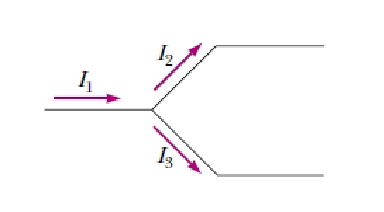
\includegraphics[width=0.3\textwidth]{./Exp2/pic/image2.png}
            \end{center}
            \caption{A Sample Junction}
            \label{fig:junction}
        \end{figure}
    \item Loop Rule: The sum of the potential differences across all elements around any closed circuit loop must be zero:
        \begin{equation}
            \sum_\text{closed loop} V = 0
        \end{equation}
        This rule simply follows from the conservation of energy.
\end{enumerate}

When applying Kirchhoff's second rule in practice, we imagine traveling around some loop and consider changes in electric potential, bearing in mind the following sign conventions:

\begin{figure}[h]
    \begin{center}
        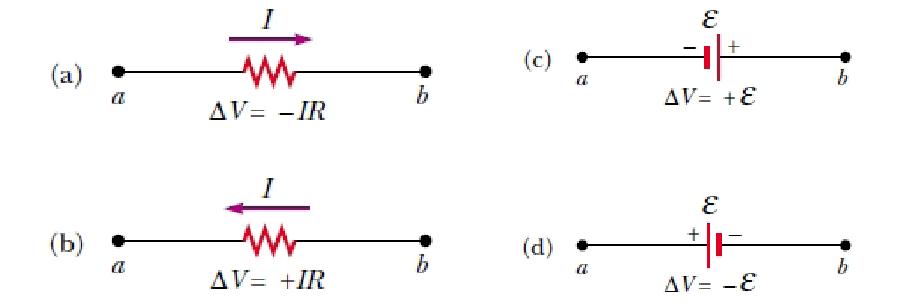
\includegraphics[width=0.6\textwidth]{./Exp2/pic/image3.png}
    \end{center}
    \caption{Sign conventions for Kirchhoff's Second Rule}
    \label{fig:kirchhoff2}
\end{figure}
\begin{itemize}
    \item If a resistor is traversed in the direction of the current, the potential difference across the resistor is negative (figure (a)).
    \item If a resistor is traversed in the direction opposite the current, the potential difference will then be negative (figure (b)).
    \item If a source of emf (assumed to have zero internal resistance) is traversed in the direction of the emf (from $-$ to $+$), the potential difference will be positive (figure (c)).
    \item If it is traversed in the direction opposite the emf (from $+$ to $-$), the potential difference will be negative (figure (d)).
\end{itemize}

In practice, for a given circuit diagram, we first label all the known and unknown quantities and assign a direction to the current in each branch of the circuit. Although the assignment of current directions is arbitrary, you must adhere rigorously to the assigned directions when applying Kirchhoff's rules. After applying Kirchhoff's rules to junctions and loops as necessary, we simply need to solve the resulting equations simultaneously for the unknown quantities. If some current turns out to be negative, that simply means that its direction is opposite to that which we assigned, but its magnitude will be correct.

\newpage
\section{Experiment}

\subsection{Setup}

A schematic diagram of the potentiometer is shown in figure \ref{fig:potcircuit}, where:

\begin{figure}[h]
    \begin{center}
        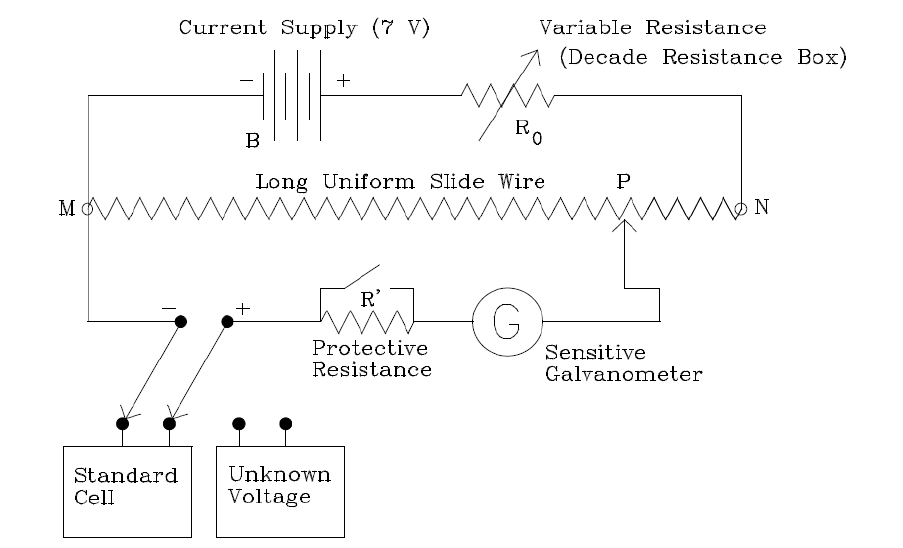
\includegraphics[width=0.8\textwidth]{./Exp2/pic/image4.png}
    \end{center}
    \caption{Circuit Diagram of the Potentiometer}
    \label{fig:potcircuit}
\end{figure}

\begin{itemize}
    \item $B$ is a stable current source with a constant voltage greater than any voltage to be measured.
    \item $MN$ is a long wire of uniform cross-section.
    \item $P$ is a sliding contact which varies the length of wire, and therefore the resistance between $M$ and $P$.
    \item $R_0$ is a decade resistance box, which is a resistor whose resistance can be varied within a certain range by turning knobs on the box. The resistance can be adjusted to reduce the total voltage across $MN$.
    \item $G$ is a sensitive galvanometer which indicates zero current when the needle deflects neither to the left nor to the right. A galvanometer is a type of ammeter (device for measuring current) that is used for direct current circuits.
    \item $R'$ is a protective resistance to limit the current through the galvanometer when the potentiometer is not balanced. The shorting button bypasses $R'$, to increase the sensitivity in determining a null current, and should be used only after an approximate balance is obtained.
\end{itemize}

\subsection{Standard Cell Calibration}\label{sec:standardcell}

Before each measurement, first adjust $R_0$, (the decade resistance box), so that the voltage across $MN$ is larger than the value of $V_x$ to be measured. Then use the standard cell to calibrate the potentiometer for this setting as described in the following paragraph.\medskip

In order to calibrate, the standard cell is connected to the circuit, and the movable contact $P$ is adjusted to a position $P_S$ at which the galvanometer reads zero. First do this with the shorting button open, and then, for a more precise reading, depress the shorting button and adjust the position of $P$ so that the galvanometer reads zero again. At this setting, the difference in potential between $M$ and $P$ is equal to the known value of $V_S$.

\subsection{Unknown Voltage}\label{sec:unknownvolt}

Next, the standard cell is replaced by a source of unknown voltage $V_x$, and the procedure is repeated to find a point $P_x$ where the galvanometer reads zero. The value of $V_x$ can then be determined from the ratio of the two distances along the slide wire ($MP_x$ and $MP_s$) along with the known value of $V_S$.\medskip

Perform this measurement for two sources of unknown voltage, first singly and then for the two cells in series. Make sure to follow the instructions in section \ref{sec:standardcell} before each measurement.\medskip

\textbf{CAUTION}: Never use a standard cell to supply current to a circuit; it is to be used only as a reference voltage when negligible current is drawn. Since drawing a large current would damage the cell, a large protective resistor has been built into the cell holder.

\subsection{Internal Resistance of a Battery}

As mentioned in the introduction, a battery can be considered as the equivalent of a source of chemical emf $\varepsilon$ in series with an internal resistance $r$. When a current $I$ is drawn from the cell, the voltage across the terminals of the cell will be $\varepsilon - Ir$. The maximum current that can be drawn from such a cell is thus $\varepsilon/r$. As a battery is used up, the value of $\varepsilon$ remains relatively constant, but the value of $r$ rises appreciably. \myskip

One way to determine $r$ would be to connect the cell to an external load, such as a light bulb, and measure both the voltage $V$ across the terminals of the cell and the current $I$ which is delivering to the load. Then the difference between $\varepsilon$, (measured in section \ref{sec:unknownvolt}), and $V$ would be $Ir$. \myskip

\begin{figure}[h]
    \begin{center}
        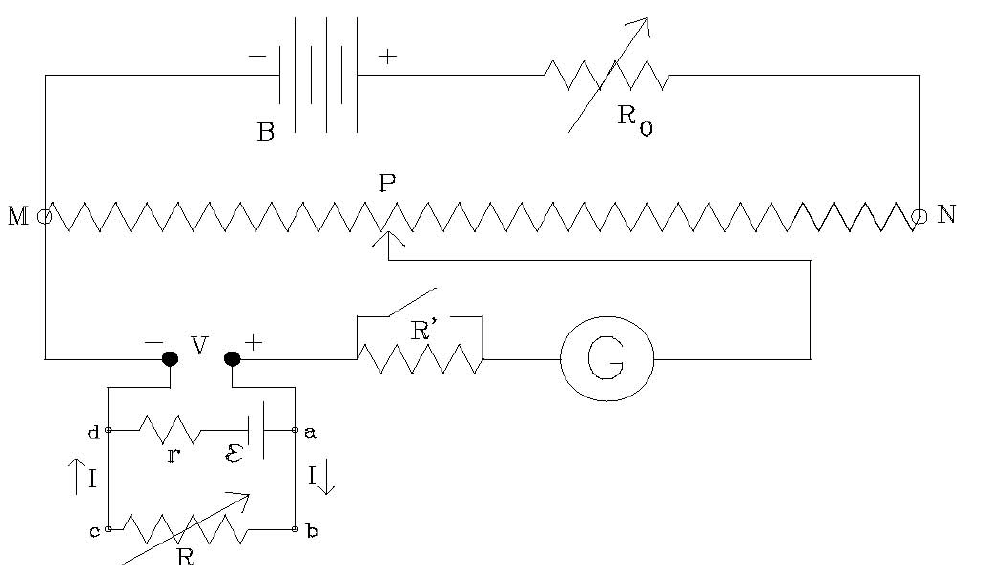
\includegraphics[width=0.8\textwidth]{./Exp2/pic/image5.png}
    \end{center}
    \caption{Circuit for Measuring Internal Resistance}
    \label{fig:internalres}
\end{figure}

However, you can alternatively determine $r$ without measuring $I$. To do this, connect a calibrated variable resistance $R$ (another decade box), as the load across the terminals to the battery, as shown in figure \ref{fig:internalres}. When $R$ is adjusted so that $V$ equals exactly half of the emf of the cell, $\varepsilon/2$, then the value of $R$ is just equal to $r$. This is so because, with the potentiometer balanced, the only current which flows in the external circuit is the current $I$ around the loop $abcd$. Thus we have the following equations:
\begin{equation}
    \varepsilon = IR + Ir,\qquad V = IR = \frac{\varepsilon}{2}
\end{equation}
Combining the above two equations we obtain:
\begin{equation}
    2IR = IR + Ir
\end{equation}
which can be simplified to yield:
\begin{equation}
    R = r
\end{equation}

To utilize this method, the best procedure is first to set $MP$ to half of the value it had for the measurement of $\varepsilon$ before $R$ was connected, that is, set the potentiometer to measure $\varepsilon /2$. Then adjust $R$ until the potentiometer is balanced at this setting.
\end{comment}
